\chapter{Результат}

%На рисунке \ref{fig:ui} представлен консольный интерфейс приложения.
%
%\begin{figure}[H]
%	\centering
%	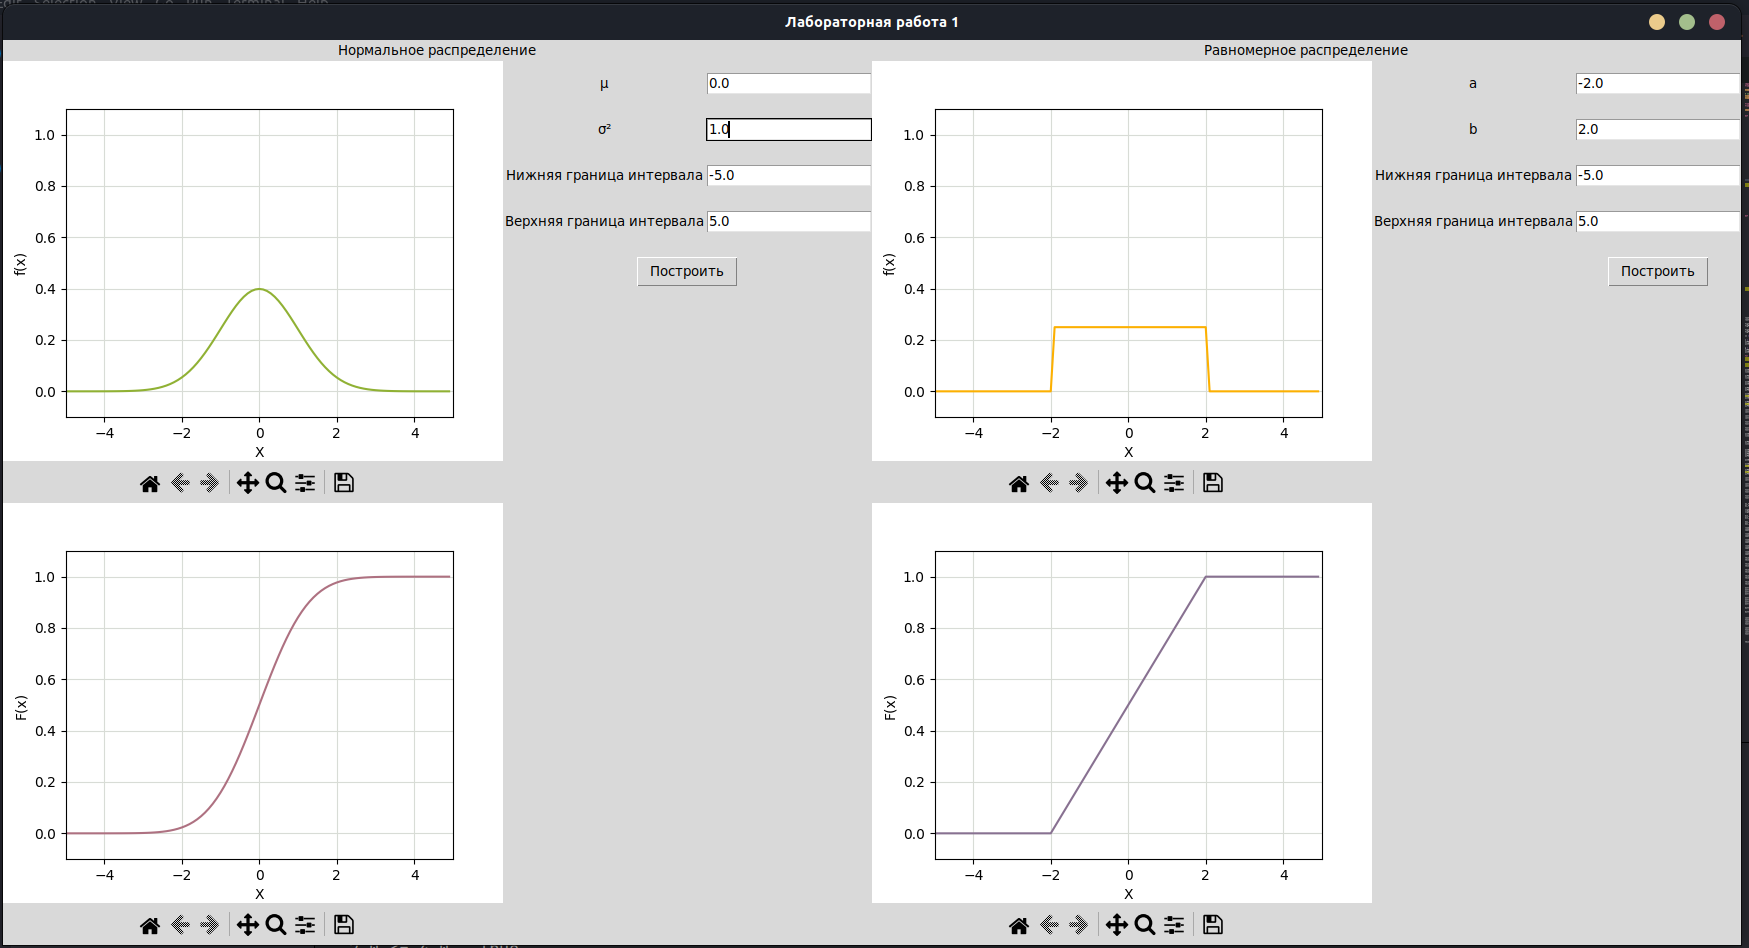
\includegraphics[width=0.7\linewidth]{assets/gui.jpg}
%	\caption{Консольный интерфейс приложения}
%	\label{fig:ui}
%\end{figure}

\section{Программный интерфейс}

Пользователю предоставляется следующие способы ввода занчений в программу:
\begin{itemize}
	\item с помощью аргументов командной строки (рис. \ref{fig:cli}), документация к которым может быть получена с помощью специальной команды (рис. \ref{fig:help})
	\item с помощью интерфейса непосредственно -- пиглашения на ввод поступают последовательно после нажатия клавиши <<Enter>> с соответсвующими комментариями (рис. \ref{fig:ui}).
\end{itemize}

\begin{figure}[H]
	\centering
	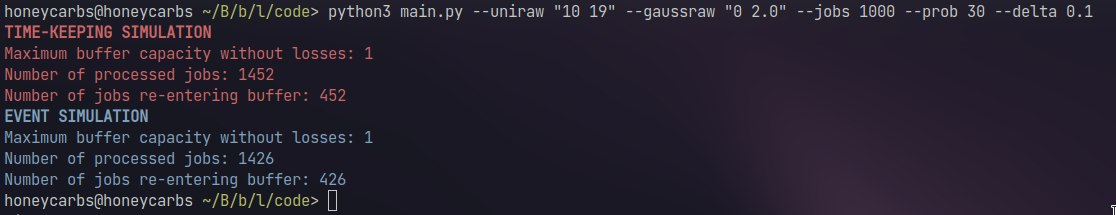
\includegraphics[width=\textwidth]{assets/cmdargs.jpg}
	\caption{Ввод данных с помощью аргументов командной строки}
	\label{fig:cli}
\end{figure}

\begin{figure}[H]
	\centering
	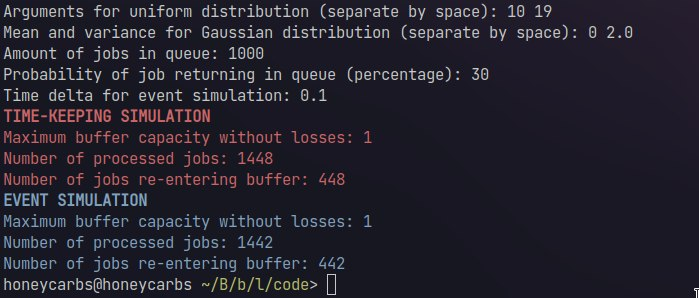
\includegraphics[width=0.9\textwidth]{assets/cli.jpg}
	\caption{Консольный интерфейс приложения}
	\label{fig:ui}
\end{figure}

\begin{figure}[H]
	\centering
	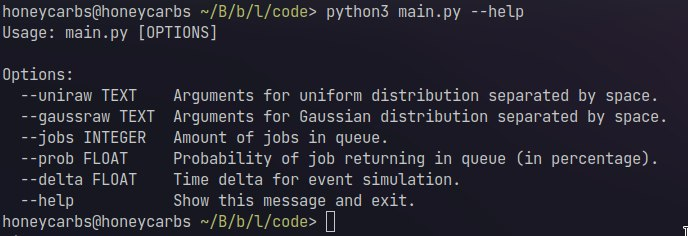
\includegraphics[width=0.7\textwidth]{assets/help.jpg}
	\caption{Информация об аргументах командной строки}
	\label{fig:help}
\end{figure}




Результат работы программы представлен на рисунках \ref{fig:cli} и \ref{fig:ui} -- результаты событийного моделирования выделены синим цветом, а пошагового -- красным.

\section{Результаты работы}

\newcolumntype{G}{>{\centering\arraybackslash}p{0.15\textwidth}}
\newcolumntype{C}{>{\centering\arraybackslash}p{0.2\textwidth}}
В таблице приведены результаты работы программы. Параметры: ${\mathcal {N}}(0 , 1.0), \; {\displaystyle {\mathcal {U}}{[1, 10]}}$, $\Delta = 0.1$.
\begin{table}[H]
	\label{tab:res}
	\caption{Результаты работы программы}
	\begin{tabular}{GGGCC}
		\hline
		\textit{модель}     & \textit{процент повторений}  & \textit{максимальное количество заявок в буфере} & \textit{обработано заявок} & \textit{количество заявок, отправленных назад в буфер} \\
		\hline 
		Событийная & \multirow{2}{*}{0}  & 1                                       & 1000              & 0                                             \\
		Пошаговая  &                     & 1                                       & 1000              & 0                                             \\ \hline
		Событийная & \multirow{2}{*}{10} & 1                                       & 1113              & 113                                           \\
		Пошаговая  &                     & 1                                       & 1103              & 103                                           \\ \hline
		Событийная & \multirow{2}{*}{40} & 2                                       & 1673              & 673                                           \\
		Пошаговая  &                     & 1                                       & 1713              & 713                                           \\ \hline
		Событийная & \multirow{2}{*}{80} & 2                                       & 4879              & 3879                                          \\
		Пошаговая  &                     & 2                                       & 5086              & 4086 \\
		\hline                                        
	\end{tabular}
\end{table}

%Программа генерирует последовательность размера 500 чисел.
%Заголовки столбцов в таблице обозначают разрядность чисел, представленных в 
%этом столбце. Заголовки строк -- номер числа в последовательности. Для алгоритмического 
%и табличного метода значения выводятся с шагом 50. Для ручного ввода выводятся все значения.
%Таблица для ручного ввода доступна к редактированию.
%
%Кнопка <<Сгенерировать>> заполняет таблицу случайно сгенерированными числами. Кнопка <<Рассчитать>>
%выводит на экран значения критериев оценки случайности для каждого столбца таблицы слева направо.
%
%Получившиеся значения представлены под таблицами. Как можно заметить, процент случайности растет с увеличением
%количества разрядов.